% Использован шаблон:
% https://www.writelatex.com/coursera/latex/1.1
% http://coursera.org/course/latex


\documentclass[a4paper,12pt]{article}

\usepackage{cmap}
\usepackage[T2A]{fontenc}
\usepackage[utf8]{inputenc}
\usepackage[english,russian]{babel}
\usepackage{fancyhdr}
\usepackage{minted}
\usepackage{hyperref}
\usepackage{amsmath}
\usepackage{graphicx}
\usepackage{xcolor}

\hypersetup{
  pdfborderstyle={/S/U/W 1}
}

\graphicspath{{./images/}}

\pagestyle{fancy}
\fancyhf{}
\lhead{Антон Завьялов, ПИ-72}
\rhead{\textbf{Лабораторная №6. Вариант 7}}
\cfoot{\thepage}

\makeatletter
\def\@seccntformat#1{%
  \expandafter\ifx\csname c@#1\endcsname\c@section\else
  \csname the#1\endcsname\quad
  \fi}
\makeatother

\begin{document} % Конец преамбулы, начало текста.

\begin{center}
  \textbf{Лабораторная работа №6 по дисциплине\linebreak"Компьютерная графика"\linebreak\linebreakВыполнил студент группы ПИ-72 Завьялов А.А.}\\
\end{center}

\section{\normalsize{Задание}}
\begin{flushleft}
    Для произвольного фотоизображения реализовать механизм коррекции и использованием фильтрации

    \begin{enumerate}
        \item искусственное наложение шума (точки, линии, окружности);
        \item сравнение фильтров шумоподавления со сменой аппертуры: равномерный и фильтр гаусса (вариант 1);
        \item сравнение методов повышения резкости;
        \item Применение спецэффектов: Акварелизация (вариант 1).
    \end{enumerate}

\end{flushleft}

\section{\normalsize{Исходный код}}
Исходный код программы также расположен в Git-репозитории по адресу: \url{https://github.com/andiogenes/cg/tree/master/image-processing}
\inputminted[breaklines]{py}{../filters.py}

\section{\normalsize{Скриншоты, демонстрирующие работу программы}}
\begin{flushleft}
  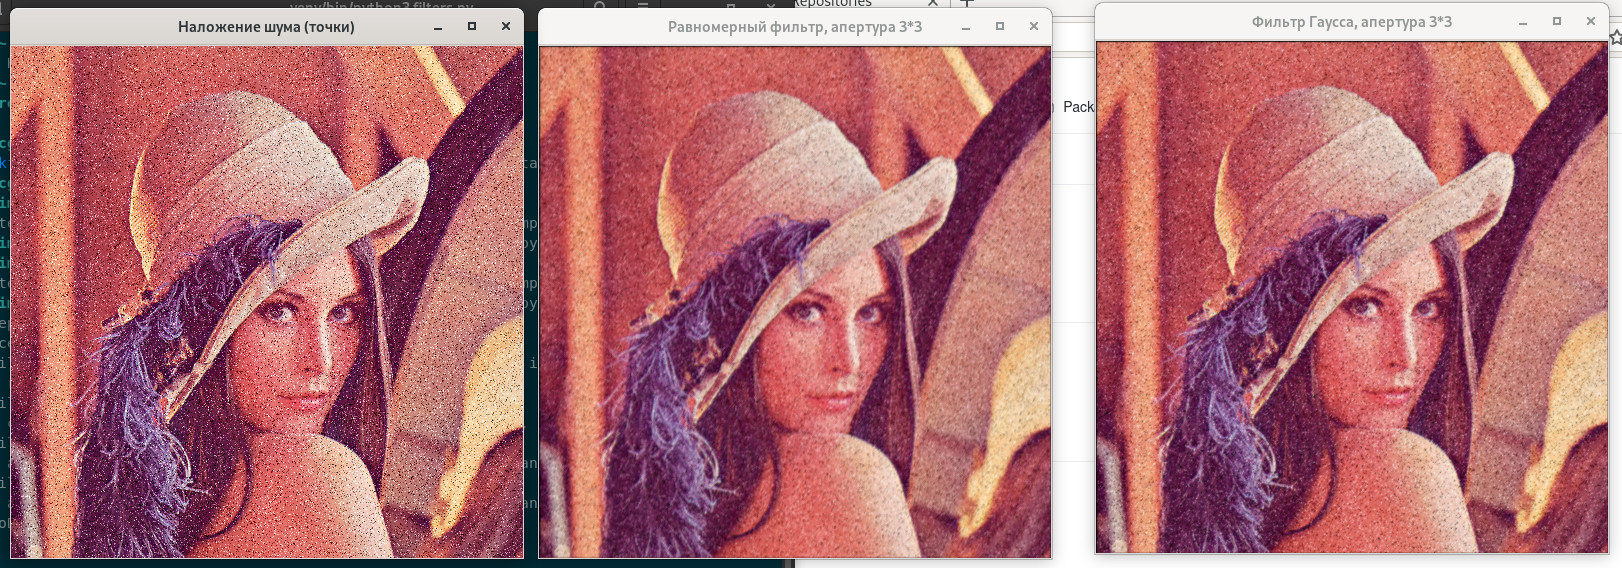
\includegraphics[scale=0.2]{blur.jpg}
  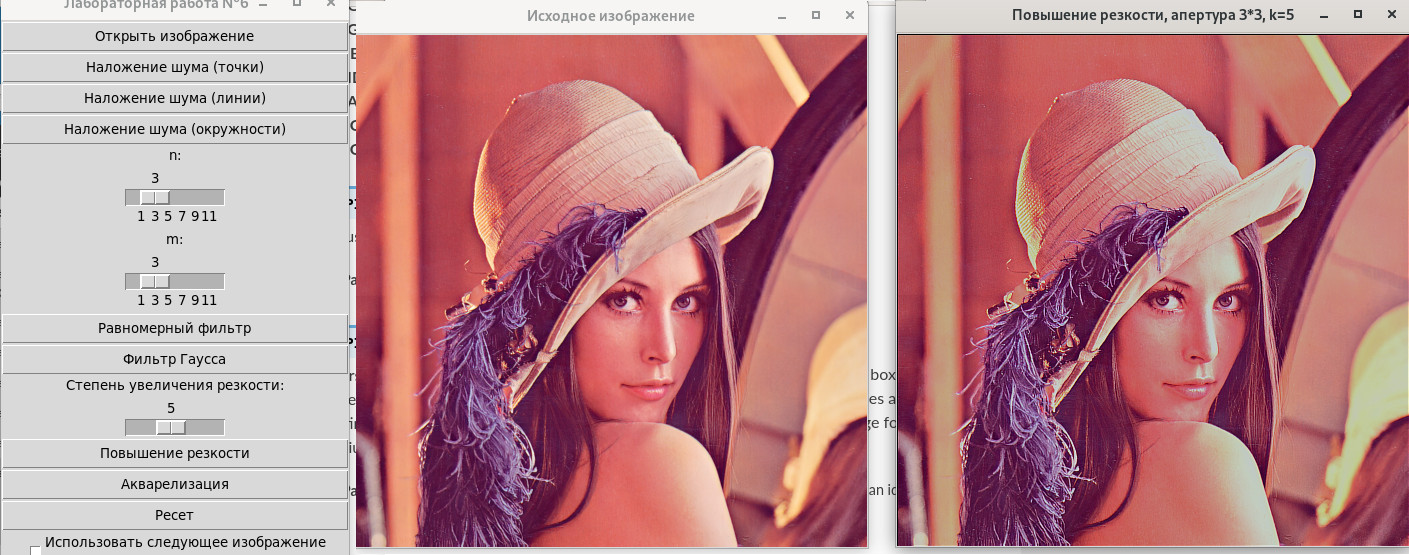
\includegraphics[scale=0.25]{sharpness.jpg}
  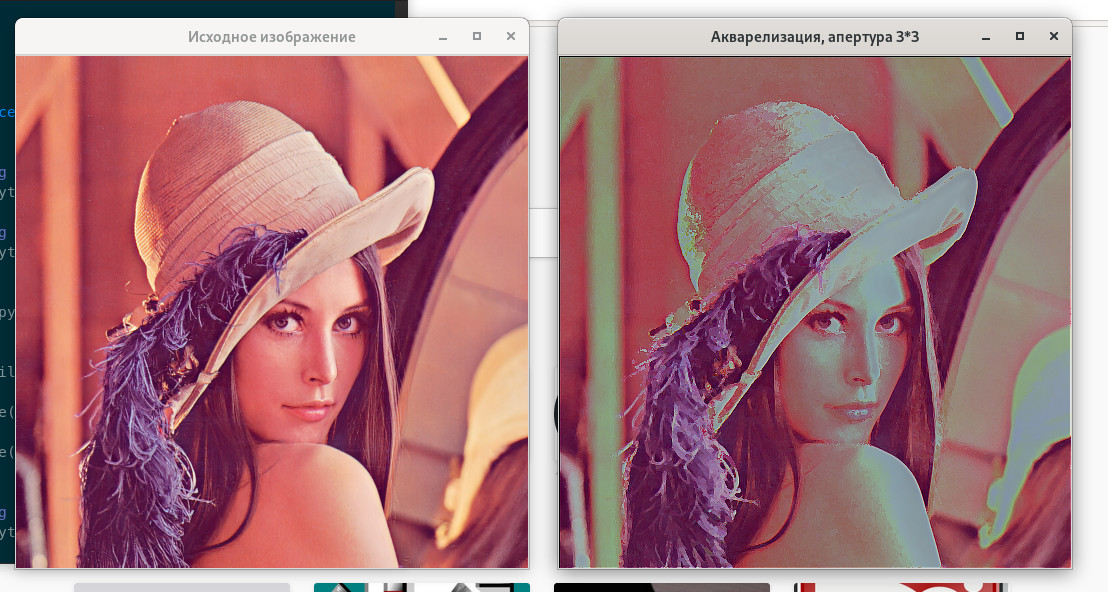
\includegraphics[scale=0.3]{watercolor.jpg}
\end{flushleft}

\end{document}

